\documentclass[10pt, letterpaper]{article}
\usepackage[brazil]{babel}    % dá suporte para os termos na língua portuguesa do Brasil
\usepackage[latin1,utf8]{inputenc}
\usepackage[T1]{fontenc}      % Lê a codificação de fonte T1 (font encoding default é 0T1).
\usepackage{ae,aecompl}
\usepackage{pslatex}
\usepackage{epsfig}
\usepackage{geometry}
\usepackage{url}
\usepackage{textcomp}
\renewcommand{\sfdefault}{lmss}
\renewcommand{\ttdefault}{lmtt}
\usepackage[table]{xcolor}
\usepackage{array}
\usepackage{longtable}
\usepackage{graphicx}
\usepackage{amsmath} 
\usepackage{wrapfig}
\numberwithin{table}{section}
\numberwithin{figure}{section}
\usepackage{color}
\usepackage{listings}


\newcommand*{\titleTMB}{\begingroup
\centering
\settowidth{\unitlength}{\LARGE MC 613}
\vspace*{\baselineskip}
{\large\scshape  Grupo 5 - Turma A}\\[\baselineskip]
\rule{11.0cm}{1.6pt}\vspace*{-\baselineskip}\vspace*{2pt}
\rule{11.0cm}{0.4pt}\\[\baselineskip]
{\LARGE Segundo laboratório }\\[0.2\baselineskip]
{\LARGE de Circuitos Digitais}\\[0.2\baselineskip]
{\itshape MC 613 - Primeiro Semestre de 2010}\\[0.2\baselineskip]
\rule{11.0cm}{0.4pt}\vspace*{-\baselineskip}\vspace{3.2pt}
\rule{11.0cm}{1.6pt}\\[\baselineskip]
{\large\scshape Professor: Guido Araújo}\par
\vfill
{\normalsize   \scshape 

\begin{center}
	\begin{tabular}{  l  l  p{5cm} }
		Henrique Serapião Gonzales     &  RA: 083636 \\
		Marcelo Galvão Póvoa & RA: 082115\\
		Tiago Chedraoui Silva      & RA: 082941\\ 
		
	\end{tabular}
\end{center}

\itshape \today }\\[\baselineskip]
\vspace{3.2pt}
\endgroup}

\begin{document}

\begin{titlepage} 
\titleTMB
\end{titlepage} 
\newpage

\newpage
\section{Quest\~ao 1:}


\newpage
\section{Quest\~ao 2:}
\lstset{language=VHDL,numbers=left, stepnumber=1,caption=Descriptive Caption Text, label=DescriptiveLabel,tabsize=3,morecomment=[l]{--},frameround=fttt,frame=trBL}
\lstinputlisting{q2a.vhdl}


\newpage
\section{Quest\~ao 3:}

Utilizando o chip 74284 projetou-se um circuito que executasse a multiplicação de 2 números de 4 bits.O chip 74284 possuía como entrada 4 bits de um número e 4 bits de do outro número, contudo retornava somente os 4 bits mais significativos da multiplicação. Para o cálculo dos 4 bits menos significativos utilizando componentes básicas do circuito lógico.
A idéia central era analisar a relevância de cada multiplicação de bits para os bits da saída.
Em que temos:
\begin{verbatim}
                            x4y0   x3y0   x2y0  x1y0  x0y0
                     x4y1   x3y1   x2y1   x1y1  x0y1
              x4y2   x3y2   x2y2   x1y2   x0y2
       x4y3   x3y3   x2y3   x1y3   x0y3
x4y4   x3y4   x2y4   x1y4   x0y4
--------------------------------------------------------------
 z8     z7     z6     z5     z4     z3     z2    z1    z0
\end{verbatim}
Como queríamos z3,z2,z1 e z0 deveriamos ter portanto:
\begin{verbatim}
z0 = x0y0
z1 = x0y1 + x1y0
z2 = x2y0 + x1y1 + x0y2
z3 = x3y0 + x2y1 + x1y2 + x0y3
\end{verbatim}
Utilizando o componente somador,usamo-lo como somadores totais (com carry na entrada) e parciais(sem carry na entrada),para o calculo dos bits menos significativos.Por exemplo,para o z1.Inicialmente como entrada no somador colocamos (x0 and y1) e (x1 and y0) sendo a sa\'ida em cm e z1 (Obs: carry e sa\'ida são usados em outros somadores, sendo o primeiro para o calculo do próximo z -nesse caso z2 - e o zm para o calculo do próprio z).

\begin{figure}[h!]
\begin{centering}
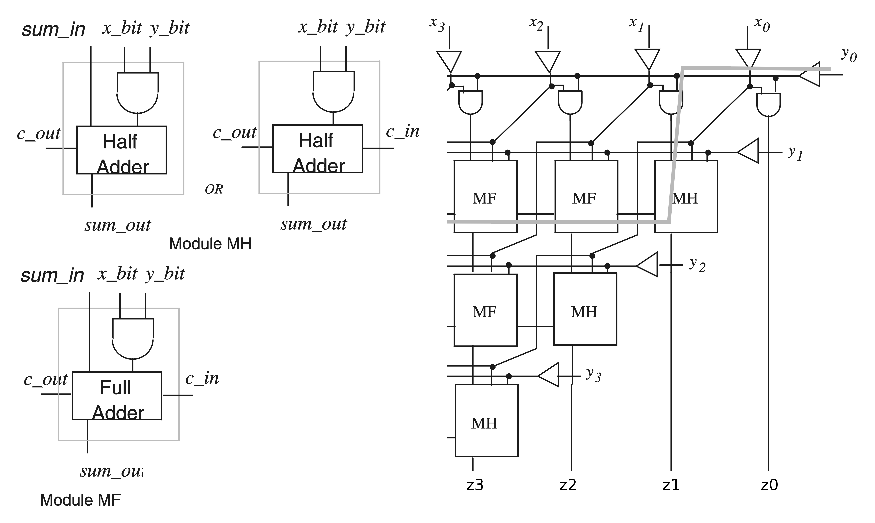
\includegraphics[scale=0.7]{q3a.eps}
\par\end{centering}
\caption{Multiplicação de 4 bits, saída dos bits menos significativos}
\end{figure}
 
Na segunda parte do projeto desenvolvemos em VHDL um multiplicador utilizando a função pré-definida {\bf y=a*b},sendo {\bf a} um inteiro de 4 bits,{\bf b} um inteiro de 4 bits e {\bf y} um vetor de 8 bits.

Posteriormente fizemos a comparação de todos os resultados possíveis através de um circuito testbench no qual simulamos todas as entradas possíveis. 
\newpage


%codigo fonte q3a%
\lstset{language=VHDL,numbers=left, stepnumber=1,caption= Multiplicador de 4 bits, label=DescriptiveLabel,tabsize=3,morecomment=[l]{--},frameround=fttt,frame=trBL}
\lstinputlisting{q3a.vhdl}


%codigo fonte q3b%
\newpage
\lstset{language=VHDL,numbers=left, stepnumber=1,caption= Funcao pre-defenida a*b, label=DescriptiveLabel,tabsize=3,morecomment=[l]{--},frameround=fttt,frame=trBL}
\lstinputlisting{q3b.vhd}

%codigo fonte q3c%
\newpage
\lstset{language=VHDL,numbers=left, stepnumber=1,caption= Comparador de resultados, label=DescriptiveLabel,tabsize=3,morecomment=[l]{--},frameround=fttt,frame=trBL}
\lstinputlisting{q3c.vhd}


\newpage
\section{Quest\~ao 4:}
\lstinputlisting{q2a.vhdl}

\hspace{0.5cm}

\end{document}






